\documentclass{article} %[letterpaper,11pt]
%\usepackage[latin1]{inputenc}
\usepackage{graphicx}
\usepackage{wrapfig}
%\usetikzlibrary{shapes,arrows}

\usepackage{amsmath}

\providecommand{\inlinecode}[1]{\texttt{#1}}

\begin{document}

\title{CS 867: Program 1}
\date{September 16, 2013}
\author{Carmen St.\ Jean}

\maketitle

\textit{Provide a written description of the way you have used visual variables to display at least three aspects of the data (approx 300-400 wds). Visual variables include such things as line width, contrast, background color, streak color, etc.}

\textit{Comment on effects. E.g., how does gray scale change affect the presentation of direction in relation to the background value. Difficulties and possible solutions may also be mentioned.}

\vspace{5 mm}

The purpose of this assignment was to create an effective flow visualization for a dataset of wind speed values.  My background is colored according to the wind speed and and my traces are colored with a single, contrasting color.  The user can right-click on the visualization to select a background color scale, select a trace color, and toggle the appearance of a legend explaining the background.

I chose to use 2,500 particles with an ``age" of 500 where each particle is advanced according to this equation:

\begin{align*} 
xp' &= xp + 0.06 dx \\
yp' &= yp + 0.06 dy
\end{align*}
where $(xp, yp)$ represents the current location of the particle, $(dx, dy)$ represents the returned value from the provided \inlinecode{getVec} function, and $(xp', yp')$ represents the new location of the particle.  The smaller coefficients of 0.06 were chosen because, combined with the age of 500, this made the flow of the particles look smooth.  For the number of particles, 2,500 was chosen because more particles led to occlusion problems while less made it harder to find the wind features.

\begin{figure}[htb]
%\begin{wrapfigure}{r}{0.4\textwidth}
   \centering
   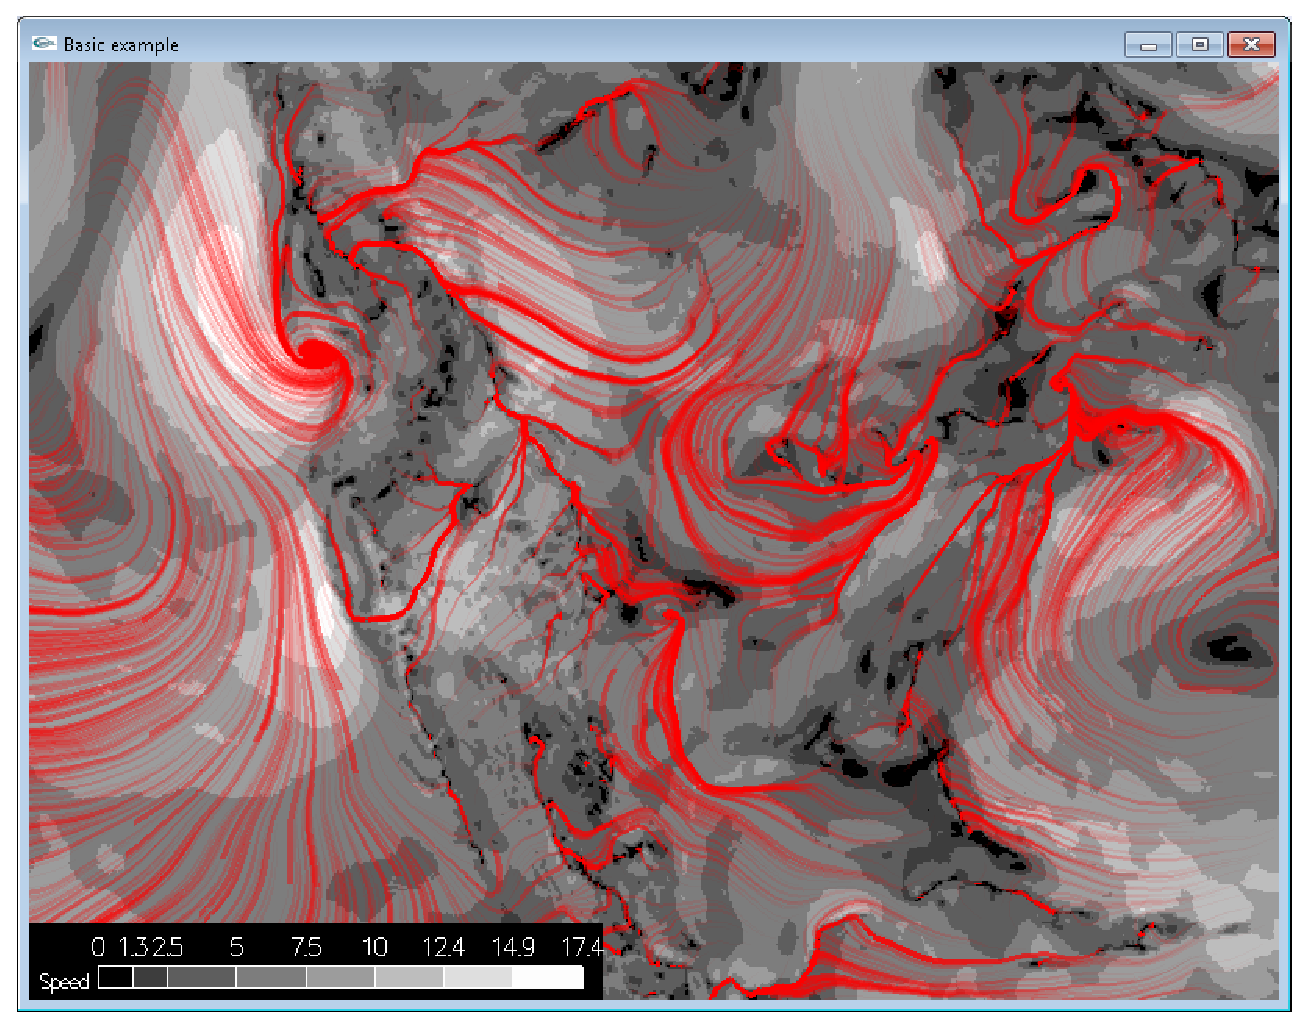
\includegraphics[height=1.2in]{images/basic_bw_red.eps}
   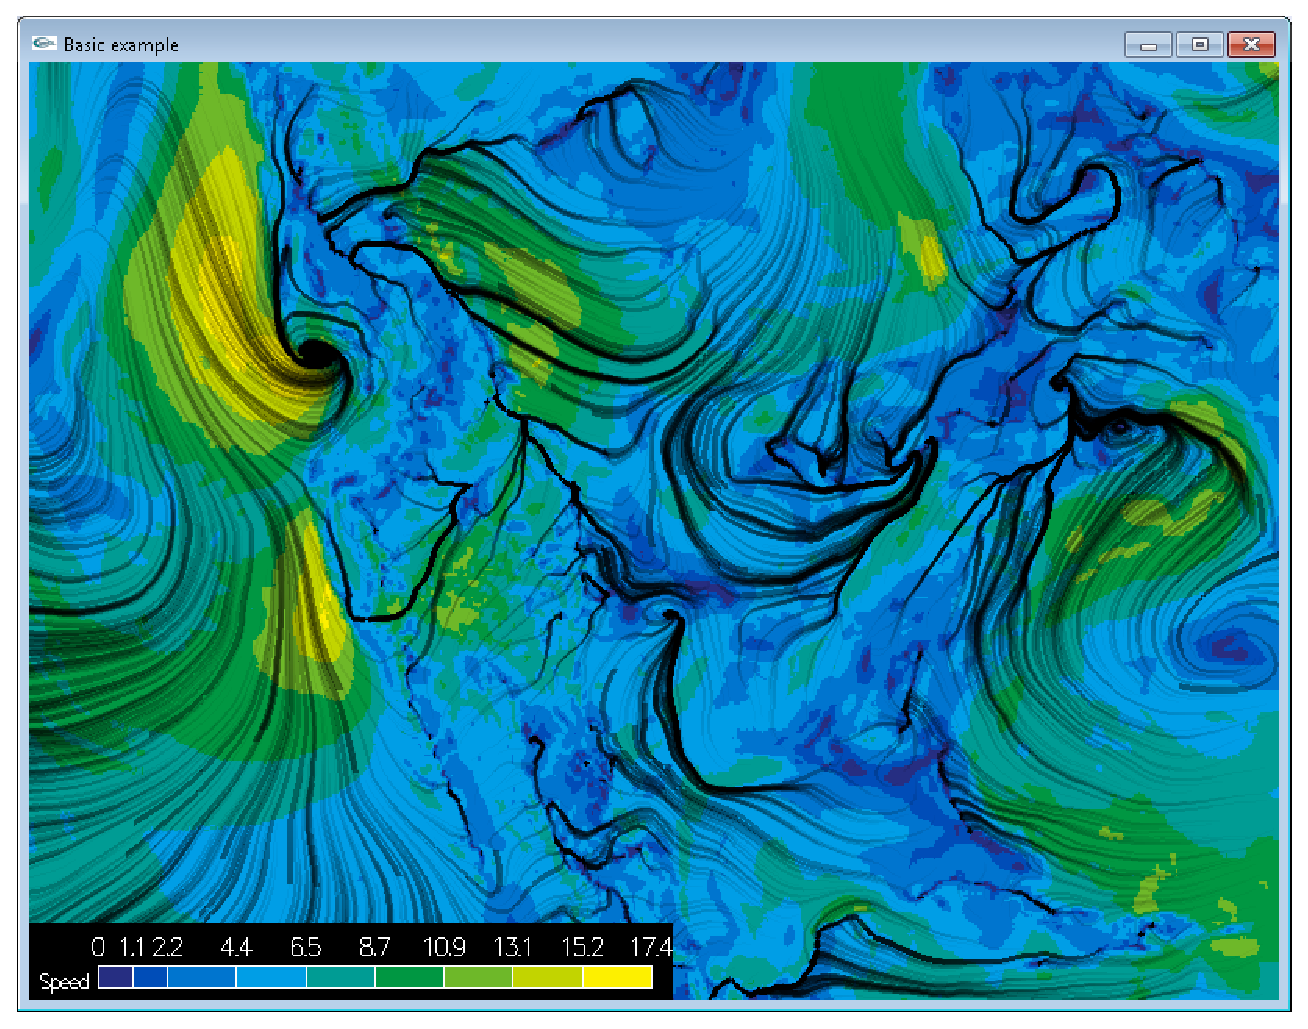
\includegraphics[height=1.2in]{images/basic_by_black.eps}
   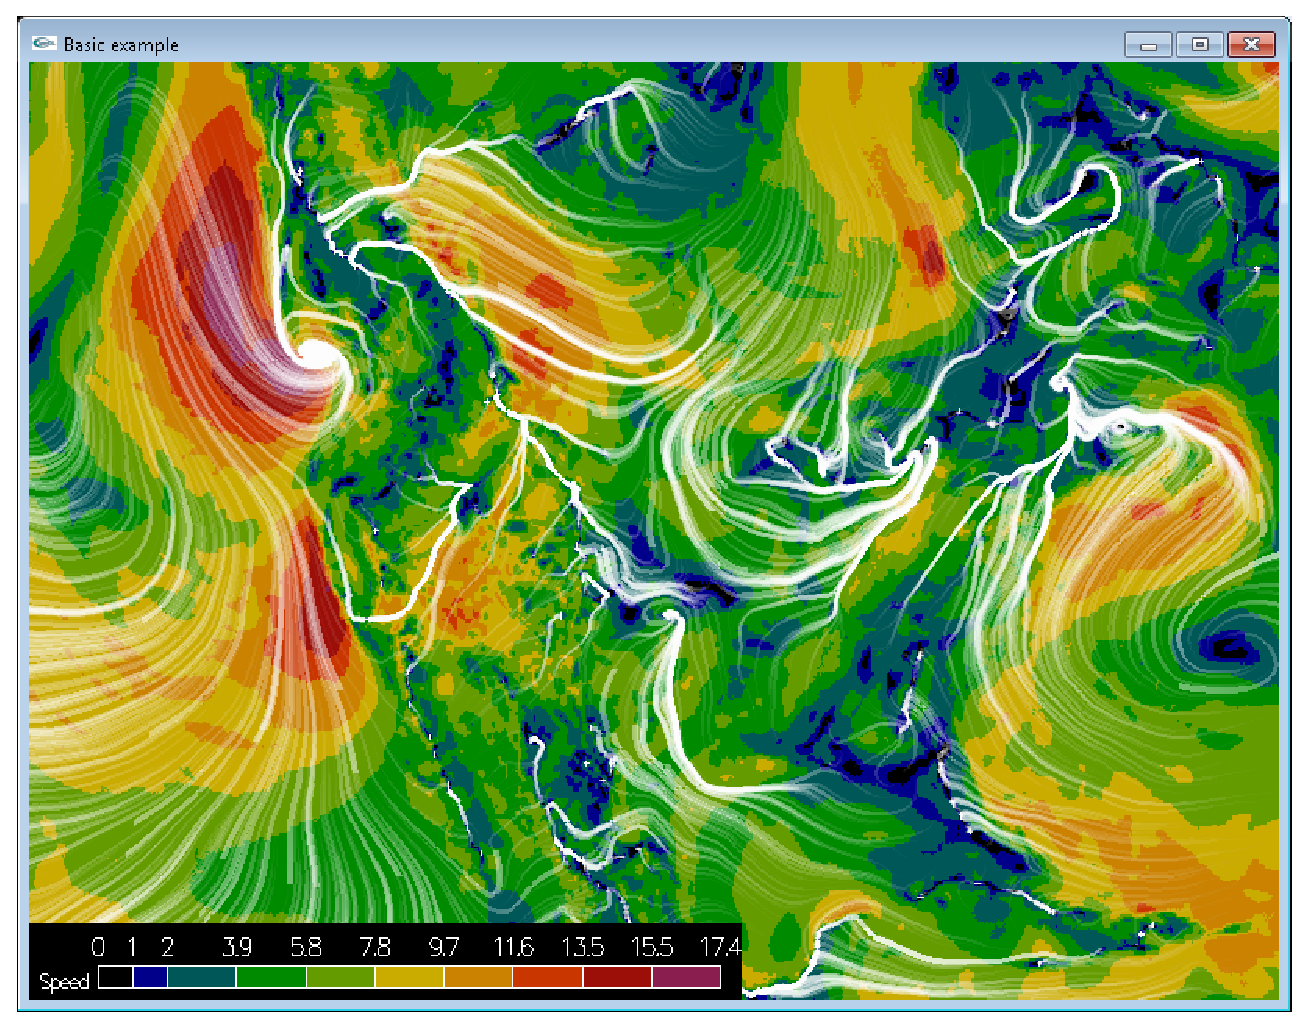
\includegraphics[height=1.2in]{images/basic_rainbow_white.eps}
    \caption{Three possible color combinations: red on black-to-white, black on blue-to-yellow, and white on rainbow.}
   \label{fig:colors}
%\end{wrapfigure}
\end{figure}

The background is colored according to the wind speed at each grid cell, with three color scale choices.  First, the rainbow background came from searching the web for various wind visualizations and finding that many used some variation of a rainbow scale.  Second, the blue-to-yellow was included because it involves neither red nor green, which most color blind people cannot distinguish.  Third, the black-to-white scale was chosen because it only varies in lightness, while the others vary in hue, lightness, and saturation, which may be confusing.

The background color scale spans from the minimum wind speed to the maximum wind speed in the dataset.  The intervals are evenly spaced according to the number of colors available, except for the first two, which are half the size of all other intervals. This allows lower speeds to be distinguished from near-zero speeds more easily.

The particle traces themselves are all colored one color -- white, black, or red.  Each of these colors can constrast against at least one background.  The ``older" end of a particle trace is thinner than the ``younger" end of the particle.  The particle trace is also more transparent (0.02 opacity) at the ``older" end than at the ``younger" end (0.45 opacity).  Therefore, the direction can be discerned by both the thickness and opacity.  The thickness of the particle trace is also increased slightly when the particle is moving faster, however this effect is not emphasized much the background encodes speed as well.

\begin{figure}[htb]
%\begin{wrapfigure}{r}{0.4\textwidth}
   \centering
   
\includegraphics[height=1.1in]{images/inwardspiral.eps}
   
\includegraphics[height=1.1in]{images/outwardspiral.eps}
   
\includegraphics[height=1.1in]{images/front.eps}
    \caption{An inward spiral, an outward spiral, and a front.}
   \label{fig:features}
%\end{wrapfigure}
\end{figure}

I found that the red on the black-to-white background is easiest to interpret, even if it does not make for the ``prettiest" picture.  However, I feel it is easiest to find the areas with the fastest winds when using the blue-to-yellow background because the yellow areas stand out.  The rainbow background is perhaps best for discerning what wind speed interval a particular grid cell falls in, but it otherwise is cluttered and confusing.

Originally, I colored the traces themselves by windspeed, but this looked confusing so I decided that one color would be better.  My traces also had an arrowhead at the ``younger" end, but this only made for clutter, especially where many traces overlapped.  I also experimented with using a continuous color scale which looked nice, but many wind scales online featured a small number of colors and intervals.

\end{document}

